\documentclass[12pt, letterpaper]{article}
\usepackage{color}
\usepackage{natbib}
\usepackage{parskip}
\usepackage{amsmath}
\usepackage{amssymb}
\usepackage{graphicx}
\usepackage{listings}
\usepackage{setspace}
\usepackage{geometry}
\usepackage{enumitem}
\usepackage{dirtytalk}
\usepackage{subcaption}
\usepackage{indentfirst}
\usepackage{anyfontsize}
\usepackage[utf8]{inputenc}

\parindent=0.5in

\graphicspath{{./imgs/}}

\definecolor{codegray}{rgb}{0.2,0.2,0.2}
\definecolor{codepurple}{rgb}{0.58,0,0.82}
\definecolor{backcolor}{rgb}{0.95,0.95,0.92}

\lstdefinestyle{scheme}
  {backgroundcolor=\color{backcolor},
  commentstyle=\color{blue},
  keywordstyle=\color{magenta},
  numberstyle=\tiny\color{codegray},
  stringstyle=\color{codepurple},
  basicstyle=\footnotesize\ttfamily,
  morekeywords={*},
  breakatwhitespace=false,
  breaklines=true,
  captionpos=t,
  keepspaces=true,
  numbers=left,
  numbersep=5pt,
  showspaces=false,
  showstringspaces=false,
  showtabs=false,
  tabsize=2,
  title=\lstname,
  language=Python
}

\lstset{style=scheme}

\doublespace{}
\title{On Splines and Their Use in Computer Graphics and Generating Curves}
\author{Simon Abrelat}
\date{\vspace{-5ex}}

\DeclareUnicodeCharacter{2212}{-}
\begin{document}

\large
{\fontsize{12}{14.4}
  {\singlespace{}
  \pagenumbering{gobble}
  \maketitle
  \begin{center}
  \vspace{4mm}
  002129--0004 \\
  \vspace{4mm}
  Math HL IA \\
  \vspace{4mm}
  May 2019 \\
  \vspace{4mm}
  Words: \\
  \end{center}
  }
}
\newpage

\pagenumbering{arabic}
\begin{abstract}
Splines are used everywhere around us, from fonts to animations. They are the way that computers deal with
curves and because of that have a large range of possible uses. Since they are so useful, there are also a
lot of ways to generate these functions and lots of formats they come in. In general, they are fairly
computationally cheap which makes them so useful and can be extended in a multitude of ways. In this paper,
the goal would be to use splines to smoothly interpolate values either for control or for path generation.
\end{abstract}

\newpage
\tableofcontents
\newpage

\section{Introduction}
Splines are not a specific equation, they are more a class of equations that have similar properties. They are
simply piecewise polynomials, and are often parameterized so that they could \say{loop over themselves} and
break the vertical line test. One of the interesting aspects of splines is that they keep this property even
at low degrees. The word spline is derived from wooden splines that curve given some constraints and are often
used in things like braces for ships. The major benefit of splines is how they are suited for computers.
Almost all curves on a computer from fonts to animation paths are described quickly and accurately by
B\`{e}zier curves and other such splines. This means that these splines are around us all of the time and are
almost invisible if you do not know where to look. There are many different kinds of splines with different
methods of formulation. However, this paper will mostly be focused on Hermite and B\`{e}zier curves.

\section{B\`ezier Curves}
\subsection{Theory}
B\`ezier curves can be made with a linear combination of Bernstein polynomials. Bernstein polynomials were
first used in the proof of the Stone-Weierstrass theorem which states that every continuous function defined
on a closed interval $[a,b]$ can be approximated as closely as desired by a polynomial \citep{weierstrass}.
A Bernstein polynomial (\ref{eq:BPoly}) is defined by a linear combination of Bernstein basis functions
(\ref{eq:BBasis}).

Bernstein Polynomials:
\begin{equation}
  \label{eq:BBasis}
  b_{\nu,n} = {n \choose \nu} x^\nu (1 - x)^{\nu - n}
\end{equation}
\begin{equation}
  \label{eq:BPoly}
  B_n(x) = \sum_{\nu = 0}^{n}\beta_\nu b_{\nu,n} (x)
\end{equation}

\begin{small}
	\begin{singlespace}
		\begin{itemize}[label=]
    	\item $\nu$: is the predicted rate for user $x$ on item $i$
    	\item $n$: is the rate of song $i$ given by user $k$
		\end{itemize}
	\end{singlespace}
\end{small}

\begin{figure}[h]
  \caption{Basis functions for different degrees}
  \label{fig:basis}
  \begin{center}
    \begin{subfigure}[b]{.45\linewidth}
      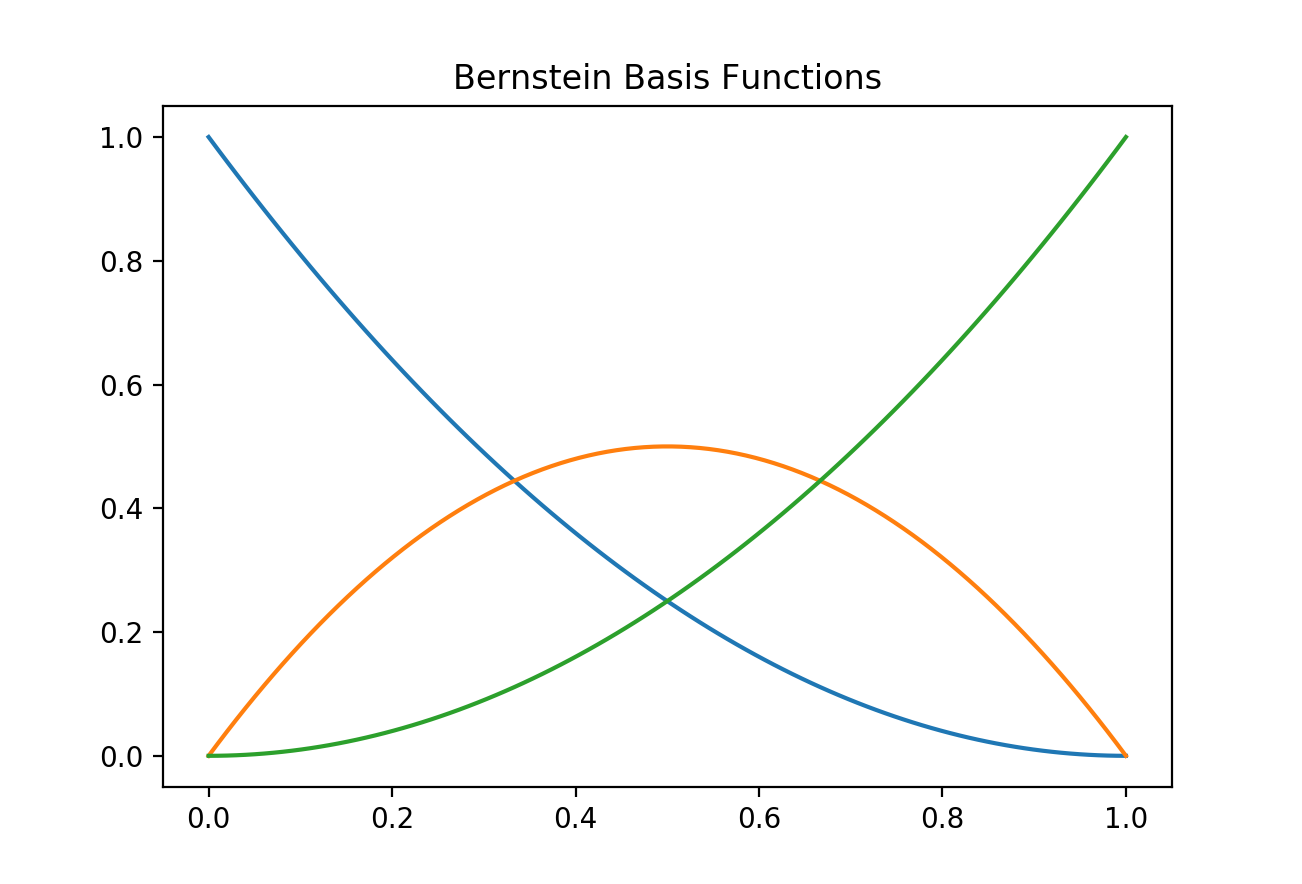
\includegraphics[width=\linewidth]{Basis/basis2}
      \caption{$n=2$}
    \end{subfigure}
    \begin{subfigure}[b]{.45\linewidth}
      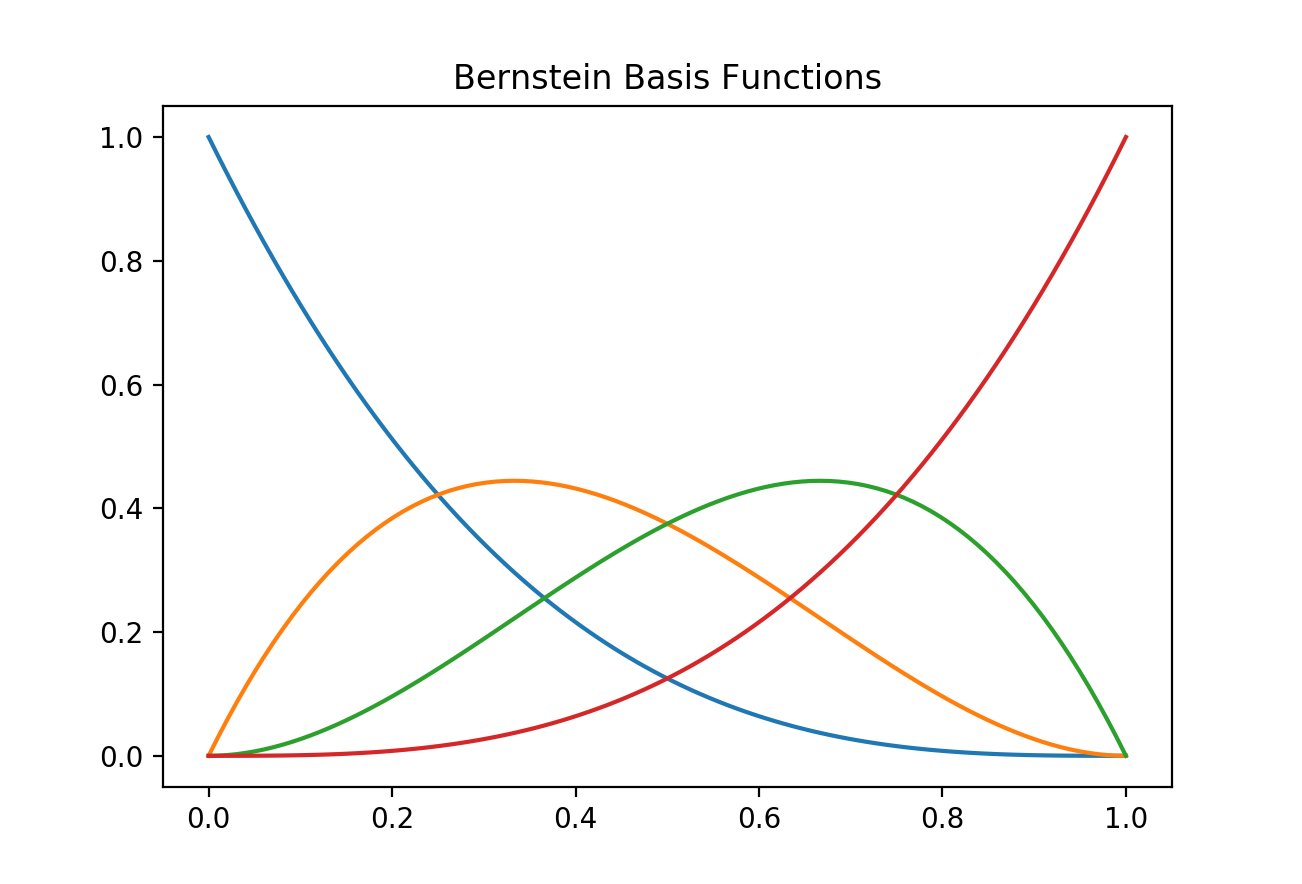
\includegraphics[width=\linewidth]{Basis/basis3}
      \caption{$n=3$}
    \end{subfigure}
  \end{center}
\end{figure}
\begin{figure}[h]
  \begin{center}
    \begin{subfigure}[b]{.45\linewidth}
      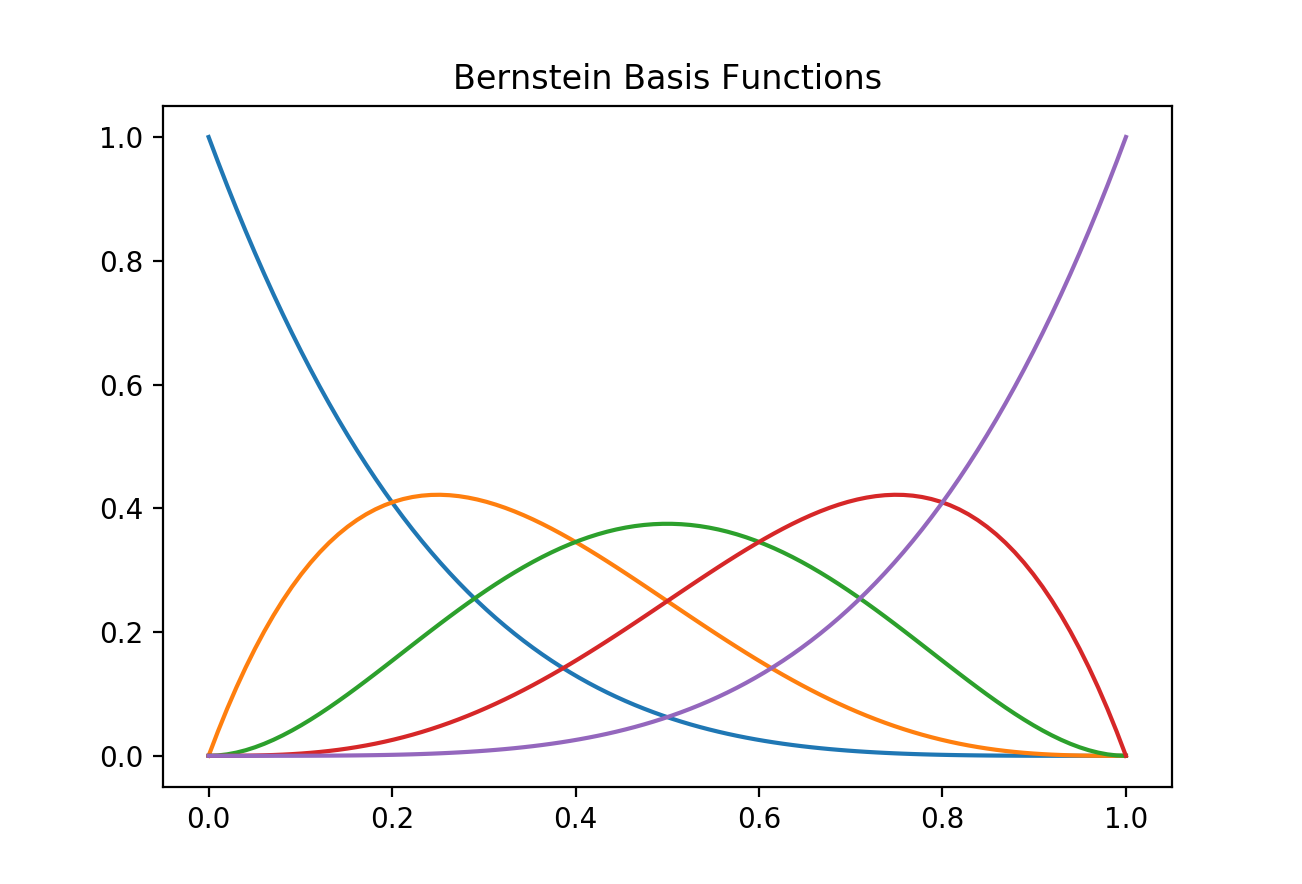
\includegraphics[width=\linewidth]{Basis/basis4}
      \caption{$n=4$}
    \end{subfigure}
    \begin{subfigure}[b]{.45\linewidth}
      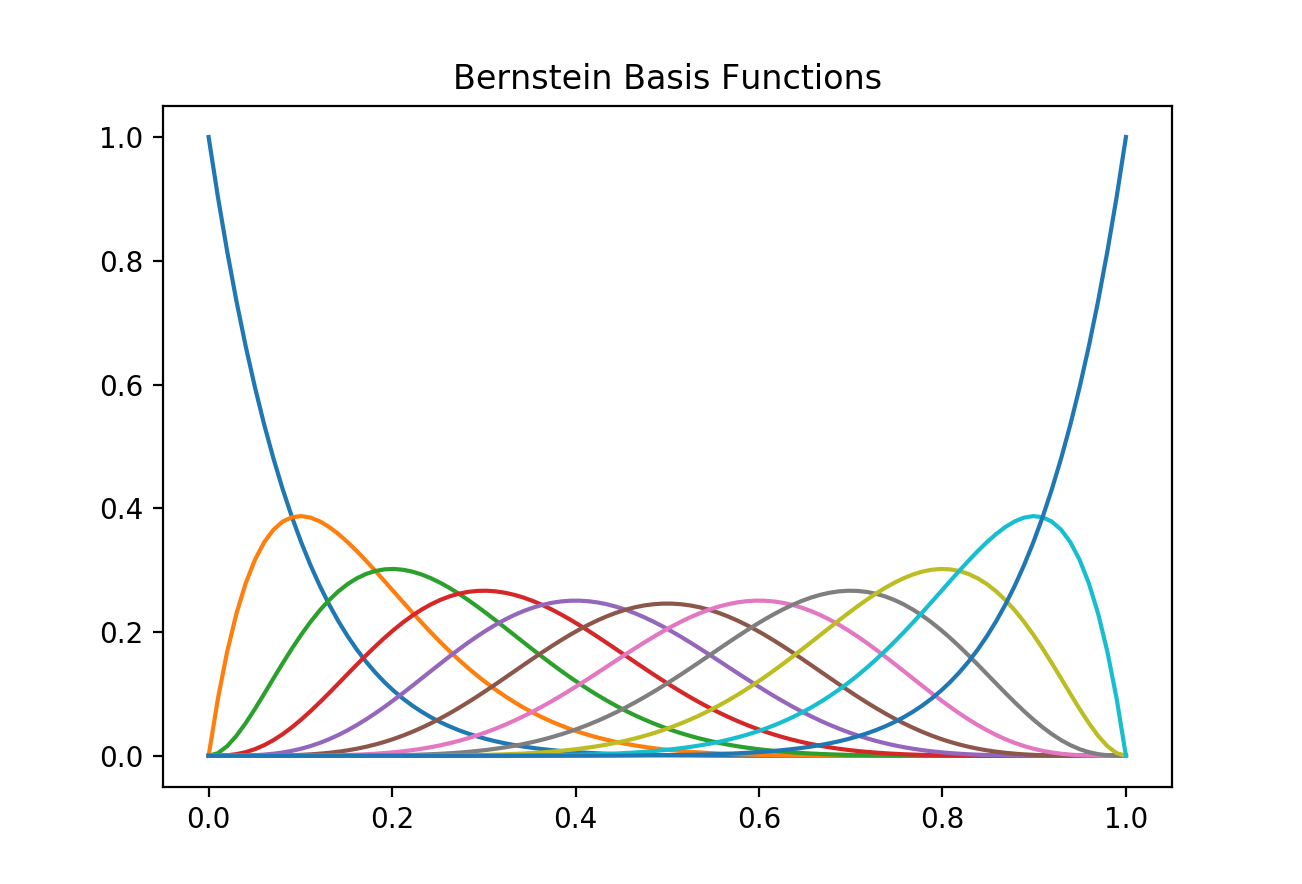
\includegraphics[width=\linewidth]{Basis/basis10}
      \caption{$n=10$}
    \end{subfigure}
  \end{center}
\end{figure}

\subsection{Application}

\bibliographystyle{apa}
\bibliography{IA}
\end{document}
